\documentclass[main]{subfiles}

\begin{document}
\begin{lect} {2019-09-17}
		\begin{utv}
		    $|G|=p$,\q $p$ - простое $\RA G \cong \Z /p \Z$
		\end{utv}

		\begin{proof}
		    $g \in G$, $g \neq e$, $\ord g=p$

		    $\Ra G=\{e=g^0,g,...,g^{p-1}\}$
		\end{proof}

		\begin{utv}
		    $H,G$ - группы, $\varphi: G \ra H$ - изоморфизм $\Ra$ $n=\ord g=\ord \varphi(g)$
		\end{utv}

		\begin{proof}
		    Пусть $g^n=e,\ \varphi(g^n)=\varphi(e)\os{?}{=}e$
		    \[\varphi(e)^2=\varphi(e^2)=\varphi(e)\]
		    Теперь докажем, что меньшего нет
		    \[\varphi(g)^m = e,\ m \in \N \os{?}{\Ra} m \geqslant n\]
			\[\varphi(g^m) = \varphi(g)^m = e = \varphi(e) \q \Ra g^m = e \Ra m \geq n\]
		\end{proof}

		\hsubsection{1.6}{Сопряжение элемента}
		\begin{definition}
		    $H<G$, тогда H - нормальная подгруппа, если $\forall h \in H, g \in G \Ra g^{-1}h g \in H$ - сопряжение элемента h с помощью элемента g, обозначается: $H \triangleleft G$
		\end{definition}

		\begin{remark}
		    Элементы подгруппы при сопряжении переходят в элементы подгруппы
		\end{remark}

		\begin{remark}
		    Подгруппа любой коммутативной группы нормальна
		\end{remark}

		\begin{example}
		    $D_3$ - 6 элементов, 3 поворота и 3 симметрии

		    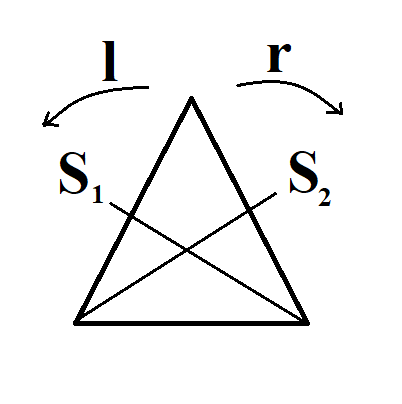
\includegraphics[width = 5cm]{pics/triangle_d_3.png}

		    $\{e,l,r\}$ - нормальная

		    $\{e, s_1\}$ - не нормальная
		\end{example}

		\begin{utv}
		    $H \triangleleft G$ $\lra$ разбиение на Л и П классы смежности по H совпадают
		    \[\forall g \q gH = Hg\]
		\end{utv}

		\begin{proof}
		    $\Ra$\\
		    \[h \in H \q g h \in g H\]
		    \[g h = \underbrace{(g^{-1})^{-1} h g^{-1}}_{\in H} g = h_1 g\]
		    $\La$\\
		    \[g \in G,\q h \in H,\q g^{-1}h g=h_1\]
		    \[h g \in H g = g H \Ra g h_1, h_1 \in H\]
		\end{proof}

		\hsubsection{1.7}{О классах смежности}
		\begin{Definition}[умножение классов смежности]
		    \[H \triangleleft G\]
		    \[g_1 H * g_2 H \eqdef g_1 g_2 H\]
		\end{Definition}

		\begin{proof}[корректности]
		    Хотим проверить, что
		    \[\w{g}_1 H = g_1 H,\q \w{g}_2 H = g_2 H \os{?}{\Ra} \w{g_1}\w{g_2}H = g_1 g_2 H\]
		    Аналогично прошлому доказательству
		    \[g_2^{-1}h_1 g_2 = h_3 \in H \]
		    \[\widetilde{g_1}\widetilde{g_2}h = g_1 h_1 g_2 h_2 h = g_1 g_2 (\us{= h_3}{g_2^{-1}h_1 g_2})h_2 h\]
		    \[\widetilde{g_1}H = g_1 H \Ra \widetilde{g}_1 = g_1 h_1\]
		    \[\widetilde{g_2}H = g_2 H \Ra \widetilde{g_2} = g_2 h_2\]
		    Не использовали условие $g_2^{-1} h_1 g_2 = h_3 \in H$
		    \[\w{g_1} \w{g_2} H = g_1 h_1 g_2 h_2 h = g_1 g_2 \us{=h_3}{(g_2^{-1} h_1 g_2) }h_2 h\]
		    Осталось доказать, что получается группа
		    \[\text{1) Нейтральный элемент}\q e H=H,\q e H * g H = (e g) H = g H\]
		    \[\text{2) Ассоциативность}\q (g_1 H+g_2 H)*g_3 H \os{?}{=} g_1 H*(g_2 H * g_3 H)\]
		    \[(g_1 g_2)H * g_3 H = (g_1 g_2)g_3 H\]
		    \[3)\q gH * g^{-1}H = (g g^{-1})H = eH \]
		\end{proof}

		\begin{Remark}
		    \[G/H\]
		    \[\text{Была эквивалентность: }a \sim b \rla a - b \ \vdots \ h\]
		    \[G = \Z\]
		    \[H=n \Z,\q g_1 g_2^{-1} \in H\text{ - мульт. запись },\q g_1-g_2 \in n \Z\text{ - адд. запись}\]
		    \[[a] + [b] = [a + b]\]
		    Аддитивная группа кольца классов вычетов - это то же самое, что фактор группа группы $\Z$ по подгруппе $n\Z$
		\end{Remark}

		\hsubsection{1.8}{Про коммутанты}
		\begin{definition}
		    Как в произвольной группе найти подгруппу?

		    $[g,h]=g h g^{-1} h^{-1}$, $g,h \in G$ - коммутатор элементов $h,g \in G$

		    Коммутант - множество произведений всех возможных коммутаторов

		    Обозначается $K(G)=\{[g_1,h_1]...[g_n,h_n],\ g_i,h_i \in G\}$
		\end{definition}

		\begin{proof}[коммутант - подгруппа]
		    $K(G)<G$\\
		    Нейтральный элемент:
				\[[e,e]=e\]
		    Обратный элемент?
				\[[g_1,h_1]...[g_n,h_n]\]
		    Как его найти?
				\[[g,h]^{-1}=(g h g^{-1} h^{-1})^{-1}=h g h^{-1} g^{-1}=[h,g]\]
		    %\[([g_1,h_1]...[g_n,h_n])^{-1}=[g_1,h_1]...[g_n,h_n]\]
            \[([g_1, h_1]...[g_n, h_n])^{-1}  = [h_n, g_n]...[h_1, g_1] \]
		    Значит это подгруппа. Нормальная ли?
				\[g^{-1}[g_1,h_1]...[g_n,h_n]g\]
				\[g^{-1} [g_1,h_1] g (g^{-1} [g_2,h_2]g)...(g^{-1} [g_n, h_n] g)\]
		    Нужно доказать, что сопряжение коммутатора лежит в коммутанте
				\[g^{-1} g_1 h_1 g_1^{-1} h_1^{-1} g =
                \underbrace{g^{-1} g_1 h_1 g_1^{-1} g h_1^{-1}}_{=[g^{-1} g_1,h_1]}
                \underbrace{h_1 g^{-1} h_1^{-1} g}_{=[h_1,g^{-1}]}\]
		\end{proof}

		\begin{utv}
		    Фактор-группа ($G / K(G)$) по коммутанту - коммутативна
		\end{utv}

		\begin{Proof}
		    \[g_1, g_2 \in G \q\q g_1 K(G) g_2 K(G) \os{?}{=} g_2 K(G) g_1 K(G)\]
            \[g_1 K(G) g_2 K (G) = g_1 g_2 K(G) \q\q g_2 K(G) g_1 K(G) = g_2 g_1 K(G)\]
			\[[g_1, g_2] = g_1 g_2 (g_2 g_1)^{-1} \in K(G) \]
		\end{Proof}

		\begin{Utv}
		    \[\Z_n \times \Z_m \simeq \Z_{mn} \text{, если } (m, n) = 1 \]
		\end{Utv}

		\begin{proof}
		    Нужно построить изоморфизм $[a]_{m n} \mapsto    ([a]_n,[a]_m)$
				\[[a]_{m n} = [a']_{m n} \Ra [a]_n = [a']_n$, $[a]_m=[a']_m\]
		    Теперь нужно проверить биекцию

		    Сюръективность:
				\[\forall b,c \in \Z$ $\e x \in \Z: \begin{cases}[x]_n=[b]_n\\ [x]_m=[c]_m \end{cases},\text{ по КТО всё хорошо}\]
		    Инъективность:
				\[\left[\begin{matrix}
						[a]_n = [b]_n\\
						[a]_m = [b]_m
				\end{matrix}\right. \RA [a]_{m n} = [b]_{m n}\]
		    На языке сравнений:
				\[\begin{matrix}
						a \equiv b(n)\\
						a \equiv b(m)
				\end{matrix} \RA a \equiv b (m n)\]
		    На самом деле достаточно было проверить одно
		\end{proof}

		\hsubsection{1.9}{Гомоморфизм}
		\begin{Definition}
				\[\varphi : G \to H \text{ - гомоморфизм, если } \varphi(g_1 g_2) = \varphi(g_1) \varphi(g_2)\]
				\[\text{изоморфизм = гомоморфизм + биекция}\]
				\[\varphi \in \text{Hom}(G, H) \text{ - множество гомоморфизмов}\]
		\end{Definition}

		\begin{Examples}
				\begin{enumerate}
						\item $\CC^* \to \R^*$
						\[z \to |z|\]
						\item $GL_n(K) \to K^*$
						\[A \to \det A\]
						\item $S_n \to  \{\pm 1\}$
						\[\sigma \to \left\{ \begin{align}
								&+1,& &\text{ если } \sigma \text{ - четн.}\\
								&-1,& &\text{ если } \sigma \text{ - неч.}
						\end{align}\]
						\item $a \in G \q G \to $
						\[g \to a^{-1}g a\]
						\[(a^{-1}g a)(a^{-1}g_1a) = a^{-1}g_1 g a\]
				\end{enumerate}
		\end{Examples}
\end{lect}
\end{document}
